\documentclass[crop,tikz]{standalone}

\usepackage{tikz}
\usepackage{anyfontsize}

\usetikzlibrary{bending}
\usetikzlibrary{arrows.meta}
\begin{document}

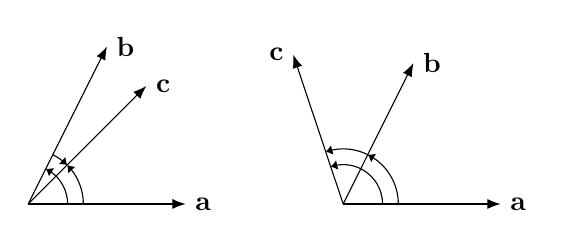
\begin{tikzpicture}
\draw [-Latex] (0,0) -- ++(1.5, 1.5);
\draw [-Latex] (0,0) -- ++(2,0);
\draw [-Latex] (0,0) -- ++(1,2);
\node [right] at (2,0) {$\bf{a}$};
\node [right] at (1,2) {$\bf{b}$};
\node [right] at (1.5,1.5) {$\bf{c}$};
\draw [arrows = {-Latex[scale length=0.5]}] ([shift=(0:0.5)]0,0) arc [radius=0.5, start angle=0, end angle= 63.5];
\draw [arrows = {-Latex[scale length=0.5]}] ([shift=(63.5:0.7)]0,0) arc [radius=0.7, start angle=63.5, end angle= 45];
\draw [arrows = {-Latex[scale length=0.5]}] ([shift=(0:0.7)]0,0) arc [radius=0.7, start angle=0, end angle= 45];

\draw [-Latex] (4,0) -- ([shift=(0:2)]4,0);
\draw [-Latex] (4,0) -- ([shift=(108.5:2)]4,0);
\draw [-Latex] (4,0) -- ([shift=(63.5:2)]4,0);
\node [right] at ([shift=(0:2)]4,0) {$\bf{a}$};
\node [right] at ([shift=(63.5:2)]4,0) {$\bf{b}$};
\node [left] at ([shift=(108.5:2)]4,0) {$\bf{c}$};
\draw [arrows = {-Latex[scale length=0.5]}] ([shift=(0:0.5)]4,0) arc [radius=0.5, start angle=0, end angle= 108.5];
\draw [arrows = {-Latex[scale length=0.5]}] ([shift=(63.5:0.7)]4,0) arc [radius=0.7, start angle=63.5, end angle= 108.5];
\draw [arrows = {-Latex[scale length=0.5]}] ([shift=(0:0.7)]4,0) arc [radius=0.7, start angle=0, end angle= 63.5];

\end{tikzpicture}

\end{document}